% Gabarit pandoc des corrigés publiés (brut et guidé). Contenu sans marque ni nom de site.
% Compilation : lualatex (latexmk -lualatex).
% Le Markdown reste la source unique : ne pas éditer ce fichier .tex à la main.
\documentclass[11pt,a4paper]{article}

% --- Moteur, polices (Latin Modern) et langue ---------------------------------
\usepackage{iftex}
\ifLuaTeX\else\errmessage{Ce document se compile avec lualatex}\fi
\usepackage{amsmath,amssymb,mathtools}
\usepackage{fontspec}
% mathrm=sym : \mathrm prend ses glyphes dans la police mathématique (ℓ, μ, Ω), comme KaTeX.
\usepackage[math-style=TeX,bold-style=TeX,mathrm=sym]{unicode-math}
% Repli pour les glyphes absents de Latin Modern (indices et exposants Unicode,
% flèches, filets des schémas en texte, symboles) : DejaVu, puis Latin Modern Math
% (ℓ, lettres mathématiques Unicode des légendes).
\directlua{
  luaotfload.add_fallback("repliTexte", {"DejaVuSerif:mode=harf;", "DejaVuSans:mode=harf;", "file:latinmodern-math.otf:mode=harf;"})
  luaotfload.add_fallback("repliMono", {"DejaVuSansMono:mode=harf;", "DejaVuSans:mode=harf;", "file:latinmodern-math.otf:mode=harf;"})
}
\setmainfont{Latin Modern Roman}[RawFeature={fallback=repliTexte}]
\setsansfont{Latin Modern Sans}[RawFeature={fallback=repliTexte}]
\setmonofont{Latin Modern Mono}[RawFeature={fallback=repliMono}]
\setmathfont{Latin Modern Math}
\usepackage[french]{babel}
\frenchsetup{SmallCapsFigTabCaptions=false}

% --- Mise en page --------------------------------------------------------------
\usepackage[a4paper,margin=2.2cm,headheight=14pt,footskip=1.2cm]{geometry}
\usepackage{microtype}
\setlength{\emergencystretch}{4em}
\tolerance=1500
\setlength{\parindent}{0pt}
\setlength{\parskip}{0.55\baselineskip plus 2pt minus 1pt}
\usepackage{xcolor}
% Gris nommés : babel-french rend « ! » actif dans le document.
\definecolor{gris2}{gray}{0.98}
\definecolor{gris3}{gray}{0.97}
\definecolor{gris5}{gray}{0.95}
\definecolor{gris35}{gray}{0.65}
\definecolor{gris40}{gray}{0.60}
\definecolor{gris45}{gray}{0.55}
\definecolor{gris50}{gray}{0.50}
\definecolor{gris55}{gray}{0.45}
\definecolor{gris60}{gray}{0.40}
\definecolor{gris65}{gray}{0.35}
\definecolor{gris70}{gray}{0.30}
\definecolor{gris80}{gray}{0.20}
\definecolor{gris85}{gray}{0.15}
\usepackage{graphicx}
\usepackage{float}
\usepackage{caption}
\captionsetup{font=small,labelformat=empty,justification=centering}
\usepackage{booktabs,longtable,array,multirow,calc}
\usepackage{siunitx}
\sisetup{locale=FR}
\usepackage[version=4]{mhchem}
\usepackage{listings}
\usepackage{fancyhdr}
\usepackage{lastpage}
\usepackage[most]{tcolorbox}
\usepackage{enumitem}
\setlist{nosep,leftmargin=*,topsep=2pt}
\usepackage[hidelinks,unicode]{hyperref}
\usepackage{bookmark}
\hypersetup{pdftitle={CCINP MPI — Mathématiques 2 2026},pdfauthor={Rédigé par IA},pdfcreator={LaTeX},pdfsubject={Corrigé brut}}
\usepackage{xurl}

% --- Pandoc : listes, tableaux, figures ----------------------------------------
\providecommand{\passthrough}[1]{#1}
\providecommand{\tightlist}{\setlength{\itemsep}{0pt}\setlength{\parskip}{0pt}}

\makeatletter
\def\maxwidth{\ifdim\Gin@nat@width>\linewidth\linewidth\else\Gin@nat@width\fi}
\def\maxheight{\ifdim\Gin@nat@height>0.55\textheight 0.55\textheight\else\Gin@nat@height\fi}
\makeatother
\setkeys{Gin}{width=\maxwidth,height=\maxheight,keepaspectratio}
\setcounter{secnumdepth}{-\maxdimen}
\providecommand{\pandocbounded}[1]{#1}

% --- Code (listings) -----------------------------------------------------------
\lstset{
  basicstyle=\ttfamily\small,
  columns=fullflexible,
  keepspaces=true,
  breaklines=true,
  breakatwhitespace=false,
  postbreak=\mbox{\textcolor{gris50}{$\hookrightarrow$}\space},
  frame=single,
  rulecolor=\color{gris35},
  framesep=4pt,
  xleftmargin=5pt,xrightmargin=5pt,
  backgroundcolor=\color{gris3},
  keywordstyle=\bfseries,
  commentstyle=\color{gris65},
  stringstyle=\color{gris80},
  showstringspaces=false,
  tabsize=4,
  extendedchars=true,
  aboveskip=6pt,belowskip=6pt,
}

% --- Macros des corrigés (KaTeX ↔ LaTeX) ---------------------------------------
% Les corrigés sont écrits pour KaTeX : on définit ici ce que KaTeX connaît et
% que LaTeX n'a pas, sans jamais retoucher le Markdown.
\providecommand{\R}{\mathbb{R}}
\providecommand{\N}{\mathbb{N}}
\providecommand{\Z}{\mathbb{Z}}
\providecommand{\Q}{\mathbb{Q}}
\providecommand{\C}{\mathbb{C}}
\providecommand{\dd}{\mathrm{d}}
\providecommand{\llbracket}{\lBrack}
\providecommand{\rrbracket}{\rBrack}
\providecommand{\lBrace}{\lbrace}
\providecommand{\rBrace}{\rbrace}
\providecommand{\Box}{\square}
\providecommand{\Diamond}{\lozenge}
\providecommand{\varnothing}{\emptyset}
\providecommand{\argmax}{\operatorname*{arg\,max}}
\providecommand{\argmin}{\operatorname*{arg\,min}}
\renewcommand{\leq}{\leqslant}
\renewcommand{\geq}{\geqslant}

% Équation hors texte : réduite à la largeur de la ligne si elle déborde.
\newsavebox{\boiteequation}
\newcommand{\equationajustee}[1]{%
  \sbox{\boiteequation}{$\displaystyle #1$}%
  \ifdim\wd\boiteequation>\linewidth
    \[\resizebox{\linewidth}{!}{\usebox{\boiteequation}}\]%
  \else
    \[#1\]%
  \fi}

% --- Encadrés pédagogiques (sobres, lisibles en noir et blanc) -----------------
\tcbset{
  encadre/.style={
    enhanced,breakable,sharp corners,
    colback=white,colframe=gris55,
    boxrule=0.4pt,leftrule=2.2pt,
    left=6pt,right=6pt,top=3pt,bottom=3pt,
    before skip=6pt,after skip=6pt,
    fonttitle=\bfseries\small,coltitle=black,
    attach title to upper,after title={\quad},
    parbox=false,
  }
}
\newtcolorbox{indication}[1]{encadre,colframe=gris45,colback=gris2,title={Indication~#1}}
\newtcolorbox{methode}{encadre,colframe=gris70,title={Méthode}}
\newtcolorbox{piege}{encadre,colframe=gris85,boxrule=0.8pt,leftrule=2.2pt,title={Piège}}
\newtcolorbox{jury}{encadre,colframe=gris60,colback=gris5,title={Jury}}
\newtcolorbox{encadrenote}{encadre,colframe=gris40}

% --- Titres de section ---------------------------------------------------------
\usepackage{titlesec}
\titleformat{\section}{\Large\bfseries}{}{0pt}{}
\titleformat{\subsection}{\large\bfseries}{}{0pt}{}
\titleformat{\subsubsection}{\normalsize\bfseries}{}{0pt}{}
\titlespacing*{\section}{0pt}{14pt plus 4pt minus 2pt}{6pt}
\titlespacing*{\subsection}{0pt}{10pt plus 3pt minus 2pt}{4pt}
\titlespacing*{\subsubsection}{0pt}{8pt plus 2pt minus 2pt}{2pt}

% --- En-tête et pied de page ---------------------------------------------------
\pagestyle{fancy}
\fancyhf{}
\fancyhead[L]{\small\textsc{Corrigé brut} · CCINP MPI}
\fancyhead[R]{\small Maths 2 2026}
\fancyfoot[L]{\footnotesize Corrigé rédigé par IA, non officiel}
\fancyfoot[R]{\footnotesize \thepage\,/\,\pageref*{LastPage}}
\renewcommand{\headrulewidth}{0.4pt}
\renewcommand{\footrulewidth}{0pt}
\fancypagestyle{plain}{\fancyhf{}\fancyfoot[R]{\footnotesize \thepage\,/\,\pageref*{LastPage}}\fancyfoot[L]{\footnotesize Corrigé rédigé par IA, non officiel}\renewcommand{\headrulewidth}{0pt}}

\begin{document}
\thispagestyle{plain}
\begin{center}
  {\small\scshape Corrigé brut}\par\smallskip
  {\LARGE\bfseries CCINP MPI — Mathématiques 2 2026\par}\medskip
  {\large CCINP · MPI · Maths 2 · 2026\par}
\end{center}
\vspace{2pt}\hrule\vspace{8pt}

\emph{Corrigé rédigé par IA, non officiel. Signalez toute erreur.}

Épreuve spécifique MPI (MPI3M2), 4 heures, calculatrices interdites. Deux exercices et un problème indépendants.

\textbf{Deux remarques sur l'énoncé}, signalées comme le N.B. y invite :

\begin{itemize}
\item
  en \textbf{Q15}, le crochet \(\langle g\mid h_n^{(n)}\rangle\) doit se lire comme l'intégrale \textbf{sans poids} \(\int_0^{+\infty}g(t)h_n^{(n)}(t)\,dt\).

  Avec le poids \(e^{-t}\) de Q12, la relation demandée est fausse : pour \(n=2\) et \(g=X^2\), on trouve \(-\frac14\) au lieu de \(4\). C'est la lecture que retient le rapport du jury ;
\item
  en \textbf{Q20}, « pour tout \(\alpha\in\mathbb R\) » doit se lire « pour tout \(\alpha>-\frac12\) » : pour \(\alpha\le-\frac12\), \(g_\alpha\notin E\).
\end{itemize}

\begin{center}\rule{0.5\linewidth}{0.5pt}\end{center}

\hypertarget{exercice-1}{%
\section{Exercice 1}\label{exercice-1}}

On note \(I=I_3\) et \(\lambda=3a+b\). On remarque que \(A=aJ+bI\) : les coefficients diagonaux valent \(a+b\), les autres \(a\).

\hypertarget{q1}{%
\subsection{Q1}\label{q1}}

Les trois colonnes de \(J\) sont égales à \(u={}^t(1,1,1)\neq0\), donc \(\operatorname{Im}J=\operatorname{Vect}(u)\) et
\equationajustee{\boxed{\operatorname{rg}J=1.}}
Par le théorème du rang, \(\dim\ker J=2\). Ainsi \(0\) est valeur propre, et \(E_0(J)=\ker J\) est le plan d'équation \(x+y+z=0\).

De plus \(Ju=3u\) avec \(u\neq0\) : \(3\) est valeur propre et \(\dim E_3(J)\ge1\).

Les sous-espaces propres associés à des valeurs propres distinctes sont en somme directe, donc \(\dim E_0(J)+\dim E_3(J)\le3\). Comme cette somme vaut au moins \(2+1\), elle vaut \(3\) : \(\dim E_3(J)=1\) et \(\mathbb R^3=E_0(J)\oplus E_3(J)\).

La somme des dimensions des sous-espaces propres vaut \(3\), donc \(J\) est diagonalisable, et
\equationajustee{\boxed{J\ \text{est semblable \text{à}}\ D=\operatorname{diag}(0,0,3).}}
Base adaptée : \({}^t(1,-1,0)\) et \({}^t(0,1,-1)\) pour \(\ker J\), puis \(u\).

\begin{figure}[H]
\centering
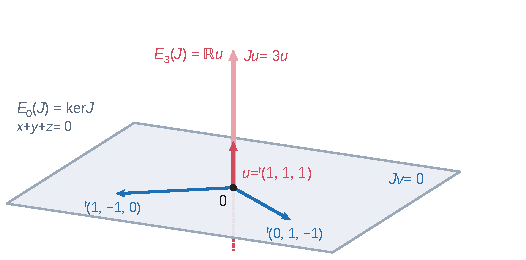
\includegraphics{figures/q1-noyau-droite-propre.pdf}
\caption*{Figure 1 --- Q1 : J annule le plan ker J d'équation x + y + z = 0 et
multiplie par 3 le vecteur u = ᵗ(1, 1, 1), orthogonal à ce plan}
\end{figure}

\hypertarget{q2}{%
\subsection{Q2}\label{q2}}

D'après Q1, il existe \(Q\in GL_3(\mathbb R)\) telle que \(Q^{-1}JQ=D\). Alors
\equationajustee{\begin{aligned}
Q^{-1}AQ&=Q^{-1}(aJ+bI)Q\\
&=aD+bI,
\end{aligned}}
donc
\equationajustee{\boxed{A\ \text{est semblable \text{à}}\ \operatorname{diag}(b,\,b,\,3a+b).}}
Ainsi \(\operatorname{Sp}(A)=\{b,\lambda\}\), avec \(E_b(A)=\ker J\) de dimension 2 et \(E_\lambda(A)=\mathbb Ru\) de dimension 1. Comme \(a\neq0\), on a \(\lambda\neq b\).

\hypertarget{q3}{%
\subsection{Q3}\label{q3}}

Les racines de \(\pi_A\) sont exactement les valeurs propres de \(A\), à savoir \(b\) et \(\lambda\), distinctes car \(a\neq0\).

Donc \((X-b)(X-\lambda)\) divise \(\pi_A\).

Par ailleurs \(A\) est diagonalisable (Q2). Une matrice est diagonalisable si et seulement si son polynôme minimal est scindé à racines simples : \(\pi_A\) est donc scindé à racines simples. Ses racines étant \(b\) et \(\lambda\), \(\pi_A\) divise \((X-b)(X-\lambda)\).

Les deux polynômes sont unitaires et se divisent mutuellement :
\equationajustee{\boxed{\pi_A=(X-b)(X-3a-b).}}

\hypertarget{q4}{%
\subsection{Q4}\label{q4}}

\textbf{a)} Soit \(n\in\mathbb N\). Comme \(\pi_A\) est de degré 2, la division euclidienne de \(X^n\) par \(\pi_A\) s'écrit
\equationajustee{X^n=S\,\pi_A+\alpha X+\beta,}
avec \(S\in\mathbb R[X]\) et \((\alpha,\beta)\in\mathbb R^2\). En évaluant en les racines \(b\) et \(\lambda\) de \(\pi_A\) :
\equationajustee{\begin{cases}b^n=\alpha b+\beta\\ \lambda^n=\alpha\lambda+\beta\end{cases}}
Par différence, \(\lambda^n-b^n=\alpha(\lambda-b)=3a\alpha\), et \(3a\neq0\). D'où
\equationajustee{\alpha=\frac{\lambda^n-b^n}{3a},}
puis
\equationajustee{\begin{aligned}
\beta&=b^n-\alpha b\\
&=\frac{\lambda b^n-b\lambda^n}{3a}.
\end{aligned}}
Comme \(\pi_A(A)=0\), on obtient \(A^n=S(A)\pi_A(A)+\alpha A+\beta I=\alpha A+\beta I\). Pour tout \(n\in\mathbb N\), avec \(\lambda=3a+b\) :
\equationajustee{\boxed{A^n=\frac{\lambda^n-b^n}{3a}\,A+\frac{\lambda b^n-b\lambda^n}{3a}\,I.}}
Contrôles : pour \(n=0\) on retrouve \(I\), pour \(n=1\) on retrouve \(A\).

\textbf{b)} Pour tous \(i,j\), \((J^2)_{i,j}=\sum_{k=1}^3J_{i,k}J_{k,j}=3\), donc \(J^2=3J\). Si \(J^k=3^{k-1}J\) pour un \(k\ge1\), alors \(J^{k+1}=3^{k-1}J^2=3^kJ\). Par récurrence :
\equationajustee{\boxed{\forall k\ge1,\quad J^k=3^{k-1}J.}}
Les matrices \(aJ\) et \(bI\) commutent, donc la formule du binôme s'applique. On isole le terme \(k=0\), où \(J^0=I\), avant d'utiliser \(J^k=3^{k-1}J\), valable seulement pour \(k\ge1\) :
\equationajustee{\begin{aligned}
A^n&=\sum_{k=0}^n\binom nk a^kb^{n-k}J^k\\
&=b^nI+\left(\sum_{k=1}^n\binom nk a^kb^{n-k}3^{k-1}\right)J\\
&=b^nI+\frac13\left(\sum_{k=1}^n\binom nk(3a)^kb^{n-k}\right)J\\
&=b^nI+\frac{(3a+b)^n-b^n}{3}\,J.
\end{aligned}}
\equationajustee{\boxed{\forall n\in\mathbb N,\quad A^n=b^n\,I+\frac{(3a+b)^n-b^n}{3}\,J.}}
Les deux résultats concordent. En reportant \(A=aJ+bI\) dans la formule du a), le coefficient de \(J\) vaut \(\frac{\lambda^n-b^n}{3}\), et celui de \(I\) vaut
\equationajustee{\begin{aligned}
\frac{b(\lambda^n-b^n)+\lambda b^n-b\lambda^n}{3a}&=\frac{b^n(\lambda-b)}{3a}\\
&=b^n.
\end{aligned}}

\begin{center}\rule{0.5\linewidth}{0.5pt}\end{center}

\hypertarget{exercice-2}{%
\section{Exercice 2}\label{exercice-2}}

On note \(\omega=\omega_1=e^{2i\pi/n}\), de sorte que \(\omega_k=\omega^k\), et \(P=\sum_{k=0}^{n-1}a_kX^k\in\mathbb R[X]\).

\hypertarget{q5}{%
\subsection{Q5}\label{q5}}

On a \(j=e^{2i\pi/3}\neq1\) et \(j^3=1\), donc \((j-1)(1+j+j^2)=j^3-1=0\) :
\equationajustee{\boxed{1+j+j^2=0.}}
Exemple : \(P=1+2X+3X^2\), de degré 2, à coefficients réels non nuls et deux à deux distincts. Ici \(n=3\), \(\omega_1=j\) et \(\omega_2=j^2=\bar j\). Avec \(j^2=-1-j\) :
\equationajustee{\begin{aligned}
P(j)&=1+2j+3(-1-j)\\
&=-2-j\\
&=-\frac32-i\frac{\sqrt3}{2}.
\end{aligned}}
Comme \(P\) est à coefficients réels, \(P(j^2)=P(\bar j)=\overline{P(j)}\), d'où
\equationajustee{\begin{aligned}
P(\omega_1)P(\omega_2)&=|P(j)|^2\\
&=\frac94+\frac34,
\end{aligned}}
\equationajustee{\boxed{P(\omega_1)P(\omega_2)=3\in\mathbb R,}}
ce qui vérifie \((*)\) sur cet exemple.

\hypertarget{q6}{%
\subsection{Q6}\label{q6}}

On a \(J_{i,j}=1\) si \(j\equiv i+1\pmod n\) et \(0\) sinon.

Pour \(x={}^t(x_1,\dots,x_n)\), cela s'écrit : \((Jx)_i=x_{i+1}\) pour \(1\le i\le n-1\), et \((Jx)_n=x_1\).

Soit \(\mu\in\mathbb C\) tel que \(\mu^n=1\), et \(v_\mu={}^t(1,\mu,\dots,\mu^{n-1})\neq0\).

Pour \(1\le i\le n-1\), \((Jv_\mu)_i=\mu^i=\mu\,(v_\mu)_i\). Enfin \((Jv_\mu)_n=1=\mu^n=\mu\,(v_\mu)_n\). Donc \(Jv_\mu=\mu v_\mu\).

Les \(n\) nombres \(\omega_0,\dots,\omega_{n-1}\) sont deux à deux distincts et vérifient \(\omega_k^n=1\).

Ce sont donc \(n\) valeurs propres distinctes de \(J\), c'est-à-dire \(n\) racines distinctes de \(\chi_J=\det(XI_n-J)\).

Ainsi \(\prod_{k=0}^{n-1}(X-\omega_k)\) divise \(\chi_J\). Ces deux polynômes, unitaires de degré \(n\), sont égaux.

Enfin \(X^n-1\) est unitaire de degré \(n\) et admet les \(n\) racines distinctes \(\omega_k\), donc \(X^n-1=\prod_{k=0}^{n-1}(X-\omega_k)\) :
\equationajustee{\boxed{\chi_J=X^n-1.}}

\hypertarget{q7}{%
\subsection{Q7}\label{q7}}

De \((Jx)_i=x_{i+1\,[n]}\) on tire par récurrence \((J^mx)_i=x_{i+m\,[n]}\). Donc \((J^m)_{i,j}=1\) si \(j\equiv i+m\pmod n\), et \(0\) sinon. Par linéarité,
\equationajustee{\begin{aligned}
\bigl(P(J)\bigr)_{i,j}&=\sum_{m=0}^{n-1}a_m(J^m)_{i,j}\\
&=a_{(j-i)\bmod n}.
\end{aligned}}
La ligne \(1\) est \(a_0,a_1,\dots,a_{n-1}\), la ligne \(2\) est \(a_{n-1},a_0,\dots,a_{n-2}\), et la ligne \(n\) est \(a_1,a_2,\dots,a_{n-1},a_0\) : c'est exactement la matrice de l'énoncé.
\equationajustee{\boxed{A=P(J).}}

\hypertarget{q8}{%
\subsection{Q8}\label{q8}}

D'après Q6, \(\chi_J=X^n-1\) est scindé à racines simples sur \(\mathbb C\). La matrice \(J\) a donc \(n\) valeurs propres distinctes, et elle est diagonalisable dans \(\mathcal M_n(\mathbb C)\) :
\equationajustee{\boxed{J=Q\,\Delta\,Q^{-1},\ \text{avec}\ \Delta=\operatorname{diag}(\omega_0,\omega_1,\dots,\omega_{n-1})\ \text{et}\ Q\in GL_n(\mathbb C).}}
On peut prendre pour \(Q\) la matrice de colonnes \(v_{\omega_0},\dots,v_{\omega_{n-1}}\).

Alors \(J^m=Q\Delta^mQ^{-1}\) pour tout \(m\), et par linéarité \(P(J)=Q\,P(\Delta)\,Q^{-1}\). Comme \(\Delta\) est diagonale, \(P(\Delta)=\operatorname{diag}(P(\omega_0),\allowbreak \dots,\allowbreak P(\omega_{n-1}))\). Avec Q7 :
\equationajustee{\boxed{A=Q\,\operatorname{diag}\bigl(P(\omega_0),P(\omega_1),\dots,P(\omega_{n-1})\bigr)\,Q^{-1}.}}
\(A\) est diagonalisable dans \(\mathcal M_n(\mathbb C)\), de valeurs propres les \(P(\omega_k)\), non nécessairement distinctes.

\hypertarget{q9}{%
\subsection{Q9}\label{q9}}

Posons \(Z=\prod_{k=1}^{n-1}P(\omega_k)\), produit vide égal à \(1\) si \(n=1\).

\emph{Déduction de Q8.} Deux matrices semblables ont même déterminant, donc
\equationajustee{\begin{aligned}
\det A&=\prod_{k=0}^{n-1}P(\omega_k)\\
&=P(1)\,Z.
\end{aligned}}
Or \(A\in\mathcal M_n(\mathbb R)\), donc \(\det A\in\mathbb R\), et \(P(1)=\sum a_k\in\mathbb R\). Si \(P(1)\neq0\), alors \(Z=\dfrac{\det A}{P(1)}\in\mathbb R\).

\emph{Cas général, y compris \(P(1)=0\).} \(P\) étant à coefficients réels, \(\overline{P(z)}=P(\bar z)\) pour tout \(z\in\mathbb C\).

Pour \(1\le k\le n-1\), \(\overline{\omega_k}=e^{-2ik\pi/n}=\omega_{n-k}\). De plus, \(k\mapsto n-k\) est une bijection de \(\{1,\dots,n-1\}\) sur lui-même. Donc
\equationajustee{\begin{aligned}
\overline Z&=\prod_{k=1}^{n-1}P(\overline{\omega_k})\\
&=\prod_{k=1}^{n-1}P(\omega_{n-k})\\
&=\prod_{k'=1}^{n-1}P(\omega_{k'})\\
&=Z.
\end{aligned}}
\equationajustee{\boxed{P(\omega_1)P(\omega_2)\cdots P(\omega_{n-1})\in\mathbb R.}}
Plus précisément, en regroupant les facteurs conjugués :

\begin{itemize}
\tightlist
\item
  si \(n\) est impair, \(Z=\prod_{1\le k<n/2}|P(\omega_k)|^2\) ;
\item
  si \(n\) est pair, \(Z=P(-1)\prod_{1\le k<n/2}|P(\omega_k)|^2\).
\end{itemize}

\begin{figure}[H]
\centering
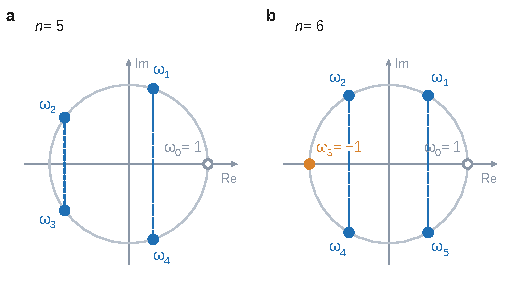
\includegraphics{figures/q9-paires-conjuguees.pdf}
\caption*{Figure 2 --- Q9 : racines n-ièmes de l'unité pour n = 5 et n = 6 ; ωₖ et
ωₙ₋ₖ sont conjugués, ω₀ = 1 n'entre pas dans le produit et, pour n pair,
−1 reste seul}
\end{figure}

\begin{center}\rule{0.5\linewidth}{0.5pt}\end{center}

\hypertarget{probluxe8me}{%
\section{Problème}\label{probluxe8me}}

\hypertarget{q10}{%
\subsection{Q10}\label{q10}}

On n'utilise que la définition de \(p_F(x)\) donnée par l'énoncé : \(E\) n'est pas supposé de dimension finie.

\textbf{a)} Soit \(y=\sum_{i=0}^n\langle x\mid e_i\rangle e_i\). C'est une combinaison linéaire des \(e_i\), donc \(y\in F\). Pour \(0\le j\le n\), par bilinéarité et orthonormalité,
\equationajustee{\begin{aligned}
\langle y\mid e_j\rangle&=\sum_{i=0}^n\langle x\mid e_i\rangle\langle e_i\mid e_j\rangle\\
&=\langle x\mid e_j\rangle,
\end{aligned}}
donc \(\langle x-y\mid e_j\rangle=0\).

Tout \(z\in F\) s'écrit \(z=\sum_j\mu_je_j\), donc \(\langle x-y\mid z\rangle=\sum_j\mu_j\langle x-y\mid e_j\rangle=0\) : \(x-y\in F^\perp\). Par unicité du vecteur de \(F\) ayant cette propriété,
\equationajustee{\boxed{p_F(x)=\sum_{i=0}^n\langle x\mid e_i\rangle\,e_i.}}

\textbf{b)} Les vecteurs \(p_F(x)\in F\) et \(x-p_F(x)\in F^\perp\) sont orthogonaux. Le théorème de Pythagore appliqué à \(x=p_F(x)+(x-p_F(x))\) donne
\equationajustee{\begin{aligned}
\|x\|^2&=\|p_F(x)\|^2+\|x-p_F(x)\|^2\\
&\ge\|p_F(x)\|^2,
\end{aligned}}
\equationajustee{\boxed{\|p_F(x)\|^2\le\|x\|^2.}}
La famille \((e_i)\) étant orthonormale, Pythagore donne aussi
\equationajustee{\begin{aligned}
\|p_F(x)\|^2&=\sum_{i=0}^n\langle x\mid e_i\rangle^2\|e_i\|^2\\
&=\sum_{i=0}^n\langle x\mid e_i\rangle^2,
\end{aligned}}
d'où
\equationajustee{\boxed{\sum_{i=0}^n\langle x\mid e_i\rangle^2\le\|x\|^2.}}

\begin{figure}[H]
\centering
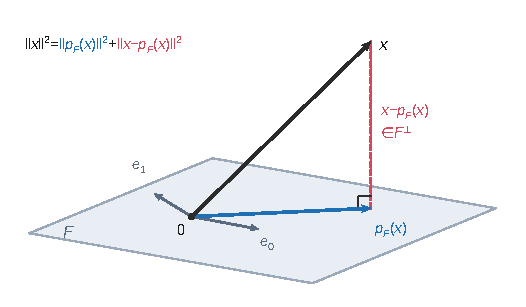
\includegraphics{figures/q10-projection-orthogonale.pdf}
\caption*{Figure 3 --- Q10 : x se décompose en p\_F(x) ∈ F et x − p\_F(x) ∈ F⊥ ;
le triangle de sommets 0, p\_F(x), x est rectangle en p\_F(x)}
\end{figure}

\hypertarget{q11}{%
\subsection{Q11}\label{q11}}

Soit \((a,b)\in\mathbb R^2\). Comme \(|a|^2=a^2\), \(|b|^2=b^2\) et \(|a||b|=|ab|\),
\equationajustee{\begin{aligned}
0&\le(|a|-|b|)^2\\
&=a^2+b^2-2|ab|,
\end{aligned}}
d'où
\equationajustee{\boxed{|ab|\le\frac{a^2+b^2}{2}.}}
Soient \(f,g\in E\). La fonction \(t\mapsto f(t)g(t)e^{-t}\) est continue sur \(I\).

Pour tout \(t\in I\), on applique l'inégalité à \(a=f(t)\) et \(b=g(t)\), puis on multiplie par \(e^{-t}>0\) :
\equationajustee{\bigl|f(t)g(t)e^{-t}\bigr|\le\frac12\Bigl(f(t)^2e^{-t}+g(t)^2e^{-t}\Bigr).}
Le majorant est intégrable sur \(I\) par définition de \(E\). Par comparaison de fonctions positives, \(t\mapsto|f(t)g(t)|e^{-t}\) est intégrable sur \(I\) :
\equationajustee{\boxed{t\mapsto f(t)g(t)e^{-t}\ \text{est \text{intégrable} sur}\ I.}}

\hypertarget{q12}{%
\subsection{Q12}\label{q12}}

\emph{\(E\) est un espace vectoriel.} On a \(E\subset\mathcal C(I,\mathbb R)\), et la fonction nulle est dans \(E\).

Soient \(f,g\in E\) et \(\mu\in\mathbb R\). La fonction \(f+\mu g\) est continue sur \(I\), et
\equationajustee{(f+\mu g)^2(t)e^{-t}=f(t)^2e^{-t}+2\mu f(t)g(t)e^{-t}+\mu^2g(t)^2e^{-t}.}
C'est une combinaison linéaire de trois fonctions intégrables sur \(I\) (définition de \(E\) et Q11), donc elle est intégrable : \(f+\mu g\in E\). Ainsi \textbf{\(E\) est un sous-espace vectoriel de \(\mathcal C(I,\mathbb R)\)}, donc un espace vectoriel.

\emph{Produit scalaire.} D'après Q11, \(\langle f\mid g\rangle\) est une intégrale absolument convergente pour tous \(f,g\in E\).

\begin{itemize}
\item
  Symétrie : \(f(t)g(t)=g(t)f(t)\), donc \(\langle f\mid g\rangle=\langle g\mid f\rangle\).
\item
  Linéarité à gauche : soient \(f_1,f_2,g\in E\) et \(\mu\in\mathbb R\). Comme \(f_1+\mu f_2\in E\), l'intégrale \(\langle f_1+\mu f_2\mid g\rangle\) converge, tout comme \(\langle f_1\mid g\rangle\) et \(\langle f_2\mid g\rangle\) (Q11).

  La linéarité de l'intégrale des fonctions intégrables donne alors
  \equationajustee{\langle f_1+\mu f_2\mid g\rangle=\langle f_1\mid g\rangle+\mu\langle f_2\mid g\rangle.}
  Avec la symétrie, l'application est bilinéaire.
\item
  Positivité : \(\langle f\mid f\rangle=\int_0^{+\infty}f(t)^2e^{-t}\,dt\ge0\), intégrale d'une fonction positive.
\item
  Caractère défini : si \(\langle f\mid f\rangle=0\), la fonction \(t\mapsto f(t)^2e^{-t}\) est \textbf{continue}, positive et d'intégrale nulle sur \(I\), donc nulle sur \(I\). Comme \(e^{-t}>0\), on obtient \(f=0\).
\end{itemize}

\equationajustee{\boxed{\langle f\mid g\rangle=\int_0^{+\infty}f(t)g(t)e^{-t}\,dt\ \text{\text{définit} un produit scalaire sur}\ E.}}

\hypertarget{q13}{%
\subsection{Q13}\label{q13}}

\emph{Inclusion \(\mathbb R[X]\subset E\).} Soit \(P\in\mathbb R[X]\). La fonction \(t\mapsto P(t)^2e^{-t}\) est continue sur \(I\).
Par croissances comparées, \(t^2P(t)^2e^{-t}\to0\) en \(+\infty\), donc \(P(t)^2e^{-t}=o(1/t^2)\).

La fonction \(t\mapsto1/t^2\) est intégrable sur \([1,+\infty[\), et la fonction étudiée est continue sur le segment \([0,1]\) : elle est intégrable sur \(I\), et \(P\in E\).

L'identification est légitime : l'application linéaire \(P\mapsto P_{\mid I}\) est injective, car un polynôme nul sur l'ensemble infini \(I\) est nul.

\emph{Structure.} \(F=\mathbb R_n[X]\) est donc une partie de \(E\). Elle contient \(0\) et elle est stable par combinaison linéaire, puisque c'est un sous-espace vectoriel de \(\mathbb R[X]\) et que les lois de \(E\) prolongent celles de \(\mathbb R[X]\). Donc
\equationajustee{\boxed{F=\mathbb R_n[X]\ \text{est un sous-espace vectoriel de}\ E,\ \text{de dimension}\ n+1.}}
De même, \(\mathbb R[X]\) est un sous-espace de \(E\), et la restriction à \(\mathbb R[X]\) du produit scalaire de Q12 est un produit scalaire sur \(\mathbb R[X]\).

\hypertarget{q14}{%
\subsection{Q14}\label{q14}}

\textbf{a)} \(h_n\) est de classe \(\mathcal C^\infty\) sur \(\mathbb R\).

Pour \(k\le n\), \((x^n)^{(k)}=\frac{n!}{(n-k)!}x^{n-k}\), et \((e^{-x})^{(q)}=(-1)^qe^{-x}\). Par la formule de Leibniz, pour \(0\le p\le n\) :
\equationajustee{\boxed{h_n^{(p)}(x)=e^{-x}\sum_{k=0}^p(-1)^{p-k}\binom pk\frac{n!}{(n-k)!}\,x^{n-k}.}}
Si \(p<n\), chaque terme contient \(x^{n-k}\) avec \(n-k\ge n-p\ge1\), donc
\equationajustee{\boxed{\forall p<n,\quad h_n^{(p)}(0)=0.}}

\textbf{b)} Avec \(p=n\), puis le changement d'indice \(m=n-k\) :
\equationajustee{\begin{aligned}
L_n(x)&=\frac{e^x}{n!}h_n^{(n)}(x)\\
&=\sum_{k=0}^n(-1)^{n-k}\binom nk\frac{x^{n-k}}{(n-k)!}\\
&=\sum_{m=0}^n(-1)^m\binom nm\frac{x^m}{m!}.
\end{aligned}}
C'est une fonction polynomiale : \(L_n\in\mathbb R[X]\). Le coefficient de \(X^n\) vaut \(\frac{(-1)^n}{n!}\neq0\). Ainsi
\equationajustee{\boxed{L_n=\sum_{m=0}^n\frac{(-1)^m}{m!}\binom nm X^m,}}
de \textbf{degré \(n\)} et de \textbf{coefficient dominant \(\frac{(-1)^n}{n!}\)}. Par exemple \(L_0=1\), \(L_1=1-X\) et \(L_2=1-2X+\frac{X^2}{2}\).

\hypertarget{q15}{%
\subsection{Q15}\label{q15}}

On lit \(\langle g\mid h_n^{(n)}\rangle\) comme \(\int_0^{+\infty}g(t)h_n^{(n)}(t)\,dt\) (voir la remarque en tête).

Soit \(g\in\mathbb R[X]\) et \(n\ge1\) ; pour \(n=0\) tout est immédiat.

Toutes les fonctions \(g^{(j)}h_n^{(m)}\) sont de la forme \(t\mapsto R(t)e^{-t}\) avec \(R\) polynomiale (Q14.a), donc intégrables sur \(I\) (argument de Q13).

Pour \(0\le j\le n-1\) et \(X>0\), une intégration par parties sur \([0,X]\), entre fonctions de classe \(\mathcal C^1\), donne
\equationajustee{\int_0^Xg^{(j)}h_n^{(n-j)}\,dt=\Bigl[g^{(j)}h_n^{(n-j-1)}\Bigr]_0^X-\int_0^Xg^{(j+1)}h_n^{(n-j-1)}\,dt.}
Le terme en \(0\) est nul car \(h_n^{(n-j-1)}(0)=0\), puisque \(n-j-1<n\) (Q14.a).

Le terme en \(X\) est de la forme \(R(X)e^{-X}\), qui tend vers \(0\) par croissances comparées. En faisant \(X\to+\infty\) :
\equationajustee{\int_0^{+\infty}g^{(j)}h_n^{(n-j)}\,dt=-\int_0^{+\infty}g^{(j+1)}h_n^{(n-j-1)}\,dt.}
En enchaînant ces \(n\) égalités, pour \(j=0,\dots,n-1\) :
\equationajustee{\boxed{\int_0^{+\infty}g(t)\,h_n^{(n)}(t)\,dt=(-1)^n\int_0^{+\infty}g^{(n)}(t)\,h_n(t)\,dt.}}
Comme \(L_n(t)e^{-t}=\frac1{n!}h_n^{(n)}(t)\) et \(h_n(t)=t^ne^{-t}\) :
\equationajustee{\begin{aligned}
\langle g\mid L_n\rangle&=\frac1{n!}\int_0^{+\infty}g(t)h_n^{(n)}(t)\,dt\\
&=\frac{(-1)^n}{n!}\int_0^{+\infty}g^{(n)}(t)\,t^ne^{-t}\,dt.
\end{aligned}}
\equationajustee{\boxed{\langle g\mid L_n\rangle=\frac{(-1)^n}{n!}\int_0^{+\infty}g^{(n)}(t)\,t^ne^{-t}\,dt.}}

\hypertarget{q16}{%
\subsection{Q16}\label{q16}}

Soient \(i<j\). La Q15 appliquée à \(g=L_i\) et à l'indice \(j\) donne
\equationajustee{\langle L_i\mid L_j\rangle=\frac{(-1)^j}{j!}\int_0^{+\infty}L_i^{(j)}(t)\,t^je^{-t}\,dt.}
Or \(\deg L_i=i<j\) (Q14.b), donc \(L_i^{(j)}=0\) et l'intégrale est celle de la fonction nulle :
\equationajustee{\boxed{\langle L_i\mid L_j\rangle=0\quad(i<j).}}

\hypertarget{q17}{%
\subsection{Q17}\label{q17}}

Soit \(I_n=\int_0^{+\infty}t^ne^{-t}\,dt\). La fonction \(t\mapsto t^ne^{-t}\) est continue sur \(I\) et, par croissances comparées, \(t^ne^{-t}=o(1/t^2)\) en \(+\infty\) : l'intégrale converge. On a \(I_0=1\).

Pour \(n\ge1\) et \(X>0\), une intégration par parties donne
\equationajustee{\int_0^Xt^ne^{-t}\,dt=-X^ne^{-X}+n\int_0^Xt^{n-1}e^{-t}\,dt.}
Comme \(X^ne^{-X}\to0\), on obtient \(I_n=nI_{n-1}\), puis par récurrence
\equationajustee{\boxed{\int_0^{+\infty}t^ne^{-t}\,dt=n!.}}
D'après Q14.b, \(L_n^{(n)}=n!\cdot\frac{(-1)^n}{n!}=(-1)^n\). La Q15 avec \(g=L_n\) donne
\equationajustee{\begin{aligned}
\langle L_n\mid L_n\rangle&=\frac{(-1)^n}{n!}\int_0^{+\infty}(-1)^nt^ne^{-t}\,dt\\
&=\frac{n!}{n!},
\end{aligned}}
\equationajustee{\boxed{\langle L_n\mid L_n\rangle=1.}}

\hypertarget{q18}{%
\subsection{Q18}\label{q18}}

Par Q16 (et symétrie) et Q17, \(\langle L_i\mid L_j\rangle=\delta_{i,j}\) : la famille \((L_0,\dots,L_n)\) est orthonormale, donc libre. Elle est formée de \(n+1\) éléments de \(F\), car \(\deg L_k=k\le n\), et \(\dim F=n+1\) :
\equationajustee{\boxed{(L_0,L_1,\dots,L_n)\ \text{est une base orthonormale de}\ F.}}
La Q10.a, appliquée dans l'espace préhilbertien \(E\) au sous-espace \(F\) de dimension finie, donne pour tout \(g\in E\) :
\equationajustee{\boxed{P_F(g)=\sum_{k=0}^n\langle g\mid L_k\rangle\,L_k,}}
où \(\langle g\mid L_k\rangle=\int_0^{+\infty}g(t)L_k(t)e^{-t}\,dt\).

\hypertarget{q19}{%
\subsection{Q19}\label{q19}}

Soit \(g\in E\).

Pour tout \(N\in\mathbb N\), \((L_0,\dots,L_N)\) est une base orthonormale de \(\mathbb R_N[X]\), sous-espace de dimension finie de \(E\) (Q13, et Q18 avec \(N\) à la place de \(n\)).

L'inégalité de Bessel (Q10.b) donne alors, pour tout \(N\in\mathbb N\),
\equationajustee{\sum_{k=0}^N\langle g\mid L_k\rangle^2\le\|g\|^2.}
La série \(\sum\langle g\mid L_n\rangle^2\) est à termes positifs, et ses sommes partielles sont majorées par \(\|g\|^2\), indépendant de \(N\). Elle converge donc, et par passage à la limite dans l'inégalité,
\equationajustee{\boxed{\sum_{n=0}^{+\infty}\langle g\mid L_n\rangle^2\le\|g\|^2,}}
où \(\|g\|^2=\int_0^{+\infty}g(t)^2e^{-t}\,dt\).

\hypertarget{q20}{%
\subsection{Q20}\label{q20}}

\emph{Appartenance à \(E\).} \(g_\alpha\) est continue sur \(I\) et \(g_\alpha(t)^2e^{-t}=e^{-(2\alpha+1)t}\).

Cette fonction est intégrable sur \(I\) si et seulement si \(2\alpha+1>0\).

Donc \(g_\alpha\in E\) \textbf{pour tout \(\alpha>-\frac12\)}, et seulement pour ceux-là : l'énoncé « pour tout \(\alpha\in\mathbb R\) » est à corriger. Pour \(\alpha>-\frac12\) :
\equationajustee{\begin{aligned}
\|g_\alpha\|^2&=\int_0^{+\infty}e^{-(2\alpha+1)t}\,dt\\
&=\frac1{1+2\alpha}.
\end{aligned}}

\emph{Coefficients.} Soit \(\alpha>-\frac12\) et \(c=1+\alpha\), de sorte que \(c>\frac12>0\).

Pour \(m\in\mathbb N\), le changement de variable \(u=ct\) (de classe \(\mathcal C^1\), strictement croissant, bijectif de \(]0,+\infty[\) sur lui-même) et Q17 donnent
\equationajustee{\int_0^{+\infty}t^me^{-ct}\,dt=\frac{m!}{c^{m+1}}.}
Avec l'expression de \(L_n\) (Q14.b) et la linéarité de l'intégrale (somme finie) :
\equationajustee{\begin{aligned}
\langle g_\alpha\mid L_n\rangle&=\sum_{m=0}^n\frac{(-1)^m}{m!}\binom nm\int_0^{+\infty}t^me^{-ct}\,dt\\
&=\frac1c\sum_{m=0}^n\binom nm\Bigl(-\frac1c\Bigr)^m\\
&=\frac1c\Bigl(1-\frac1c\Bigr)^n,
\end{aligned}}
\equationajustee{\boxed{\langle g_\alpha\mid L_n\rangle=\frac{\alpha^n}{(1+\alpha)^{n+1}}.}}

\emph{Somme.} On a \(\langle g_\alpha\mid L_n\rangle^2=\frac{q^n}{(1+\alpha)^2}\), avec \(q=\frac{\alpha^2}{(1+\alpha)^2}\). Or \((1+\alpha)^2-\alpha^2=1+2\alpha>0\), donc \(0\le q<1\) et la série géométrique converge :
\equationajustee{\begin{aligned}
\sum_{n=0}^{+\infty}\langle g_\alpha\mid L_n\rangle^2&=\frac1{(1+\alpha)^2}\cdot\frac1{1-q}\\
&=\frac1{(1+\alpha)^2-\alpha^2}\\
&=\frac1{1+2\alpha}.
\end{aligned}}
\equationajustee{\boxed{\sum_{n=0}^{+\infty}\langle g_\alpha\mid L_n\rangle^2=\|g_\alpha\|^2.}}
L'inégalité de Bessel de Q19 est une égalité pour \(g_\alpha\) : c'est l'égalité de Parseval pour la famille de Laguerre sur cet exemple.

\textbf{FIN}

\end{document}
